% Definition der Klasse des Dokumentes
\documentclass[11pt, a4paper]{article}

\usepackage[T1]{fontenc}        % Sorgt u.a. dafür, dass Texte vernünftig markierbar werden auch bei Sonderzeichen
\usepackage{ae,aecompl} %bessere Schrift
\usepackage{gensymb}
\usepackage[ngerman]{babel}     % Deutsches Wörterbuch usw.
\usepackage{epstopdf}   % Wandelt .eps Dateien automatisch um
\usepackage{url}    % für URL mit \url{.....}
\usepackage[font=small,labelfont=bf]{caption}       % Optionen für Bild- und Codeunterschriften
\usepackage[hidelinks]{hyperref}                    % damit Links in der PDF anklickbar werden
\usepackage{booktabs}   % bessere Tabellen mit Abstand zur hline
\pagenumbering{arabic}
\usepackage[babel,german=guillemets]{csquotes} %deutsches Anführungszeichen
\usepackage{float} %bessere Positionierungsoptionen

% Standardpakete für deutsche Sprache
\usepackage[utf8]{inputenc}
\usepackage[ngerman]{babel}

% Volle Seite nutzen
\usepackage{fullpage} 
\headsep 1cm
\parindent 0cm

% einige Pakete für Mathematische Darstellung
\usepackage{amssymb, amstext, amsmath}
\usepackage{fancyhdr}

% ein Paket für die Zählung von Seiten
\usepackage{count1to}
\usepackage{lastpage} 

%Paket für Aufzählungsbuchstaben
\usepackage{enumitem}

% HIER DIE NAMEN UND EMAIL ANPASSEN
\def \ATutantName{Moritz Breipohl}
\def \ATutantEmail{mbreipohl@techfak.uni-bielefeld.de}
\def \BTutantName{Markus Rothgänger}
\def \BTutantEmail{mrothgaenger@techfak.uni-bielefeld.de}
% HIER DIE VERSUCHSNUMMER ANPASSEN
\def \Versuchsnummer{Versuch 2}
% HIER DIE GRUPPENNUMMER ANPASSEN
\def \Gruppennummer{Gruppe 5}
% HIER DEN TUTORNAMEN ANPASSEN
\def \Tutorname{Lukas Schmidt, Robin Ewers}

% Kopfzeile und Fußzeile
\lhead{\Versuchsnummer}
\chead{\textbf{Digitalelektronisches Praktikum}}
\rhead{\today}
\lfoot{\Gruppennummer}
\rfoot{\thepage\ von \pageref{LastPage}}
\cfoot{}

% Wird zur Einbindung von Bildern benötigt
\usepackage{graphicx}
\graphicspath{{images/}}

% Physikalische Einheiten darstellen
\usepackage{siunitx}

% Einbinden des Literaturverzeichnisses
\usepackage[style=numeric-comp]{biblatex}
\bibliography{literatur.bib}

% Wird zum Einbinden von LaTeX Code benötigt
\usepackage{color}
\usepackage{showexpl}
\lstset
{
    language=[LaTeX]TeX,
    breaklines=true,
    basicstyle=\tt\scriptsize,
    keywordstyle=\color{blue},
    identifierstyle=\color{magenta},
}

\renewcommand{\footrulewidth}{0.4pt}
\pagestyle{fancy}

% Konfiguration des Deckblatts
\begin{titlepage}
\title{\textbf{Digitalelektronisches Praktikum\\ Versuch 3}}
\author{\ATutantName \\ \emph{\ATutantEmail} \and \BTutantName\\ \emph{\BTutantEmail}}
\date{\Gruppennummer \\[3ex] Tutor: \Tutorname \\[3ex] \today}
\end{titlepage}

\begin{document}
% Einfügen des Deckblatts
\clearpage
\maketitle
\thispagestyle{empty}
\newpage

%%%%%%%%%%%%%%%%%%%%%%%%%%%%%%%%%%%%%%%%%
%%% Ab hier Beginn des Laborberichts: %%%%%%%%%%%%%%%%%%%%%

\section*{Versuchsaufbau}
\subsection*{Aufgabe}
Ziel des Versuches war es MOS-Transistoren zu untersuchen indem für einen Typ (N-MOS) dessen Eingans- und Ausgangskennlinie erfasst wurde. Dabei war der Unterschied von N-MOS zu P-MOS Transistoren herauszustellen. 
\subsection*{Aufbau}
\begin{figure}
    \centering
    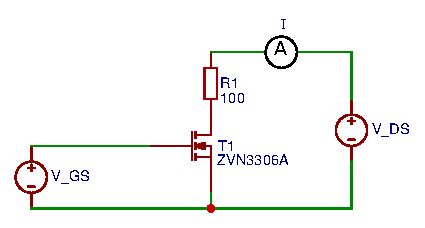
\includegraphics[width=\linewidth]{aufbau.pdf}
    \caption{Versuchsaufbau}
    \label{versuchsaufbau}
\end{figure}
Das erste Netzteil wurde am Transistor am Gate-Source-Eingang angelegt und die Spannung zur Feststellung der Eingangskennlinie schrittweise erhöht. Am Drain-Source Eingang wurde ein weiteres Netzteil angeschlossen, an welchem die Spannung zur Festlegung der Ausgangskennlinie schrittweise erhöht wurde. Am jeweils anderen Netzteil wurde die Spannung konstant gelassen und ggf. nachgeregelt. Im Drain-Source Schaltkreis wurde ein Widerstand und das Ampermeter in Reihe geschaltet. Der Aufbau ist in \autoref{versuchsaufbau} zu sehen.
\subsection*{Verwendete Bauteile}
Multimeter, N-MOS Transistor ZVN3306A, $100 \Omega$ Widerstand, zwei Netzteile mit begrenztem Strom von $0.1 A$.
\section*{Durchführung}
Im ersten Versuchsteil sollte die Eingangskennlinie des Transistors (hier N-MOS) bestimmt werden. Dazu wurde die Drain-Source Spannung konstant gehalten und die Gate-Source Spannung schrittweise erhöht während der Strom im Drain-Source Schaltkreis gemessen wurde. Beendet wurde die Messung, konnte keine signifikante Veränderung des Stroms festgestellt werden.
Im zweiten Teil wurde die Ausgangskennlinie erfasst, indem die Gate-Source Spannung konstant gehalten wurde, während die Drain-Source Spannung schrittweise erhöht wurde. Der Versuch wurde für zwei verschiedene Gate-Source Spannungen durchgeführt.
In beiden Teilen war mit jeder Spannungsveränderung darauf zu achten, dass die konstante Spannung gegebenenfalls nachjustiert werden musste.
\section*{Messergebnisse}
Zur Bestimmung der Eingangskennlinie wurde die Drain-Source Spannung auf $U_{DS} = 3 V$ geregelt. Für niedrige Spannungen im Gate-Source Kreis war kein Stromfluss zu erkennen, daher wurden die Messergebnisse zwischen $U_{GS} = 0.2 V$ und $U_{GS} = 1.9 V$
vernachlässigt. Hier ist ein Stromfluss von $I = 0 mA$ anzunehmen. Die Vollständigen Messergebnisse der Eingangskennlinie sind in \autoref{eingangskennlinie} dargestellt.
\begin{table}[h]
\centering
\begin{tabular}{c|c}
$U_{GS} [V]$ & $I [mA]$ \\ \hline
$0$ 	& $0$ \\
$0.1$ 	& $0$ \\
$0.2$ 	& $0$ \\
$1.9$	& $0.241$ \\
$2.0$	& $0.67$ \\
$2.1$	& $1.518$ \\
$2.2$	& $3.054$ \\
$2.3$	& $5.162$ \\
$2.4$	& $7.765$ \\
$2.5$	& $10.96$ \\
$2.6$	& $14.28$ \\
$2.7$	& $17.83$ \\
$2.8$	& $21.37$ \\
$2.9$	& $23.34$ \\
$3.0$	& $24.1$ \\
$3.1$	& $24.5$ \\
$3.2$	& $24.72$
\end{tabular}
\caption{Messung der Eingangskennlinie}
\label{eingangskennlinie}
\end{table}
Zur Bestimmung der Ausgangskennlinie wurde die Gate-Source Spannung auf $U_{GS} = 3 V$ im ersten, und auf $U_{GS} = 2.5 V$ im zweiten Durchgang geregelt. Die Messwerte sind in \autoref{ausgang3V} und \autoref{ausgang2-5V} dargestellt.
\begin{table}[htb]
    \centering
    \begin{minipage}[b][][b]{0.45\linewidth}
        \centering
		\begin{tabular}{c|c}
		$U_{DS} [V]$ & $I [mA]$ \\ \hline
		$0.0$ & $0.0$ \\
		$0.2$ & $1.59$ \\
		$0.4$ & $3.178$ \\
		$0.6$ & $4.729$ \\
		$0.8$ & $6.193$ \\
		$1.0$ & $7.644$ \\
		$1.2$ & $8.857$ \\
		$1.4$ & $9.821$ \\
		$1.6$ & $10.34$ \\
		$1.8$ & $10.56$ \\
		$2.0$ & $10.66$ \\
		$2.5$ & $10.79$ \\
		$3.0$ & $10.90$ 
		\end{tabular}
		\caption{Messung der Ausgangskennlinie bei $U_{GS} = 3 V$}
		\label{ausgang3V}
    \end{minipage}% 
    \hfill
    \begin{minipage}[b]{0.45\linewidth}
        \centering
		\begin{tabular}{c|c}
		$U_{DS} [V]$ & $I [mA]$ \\ \hline
		$0.0$ & $0.0$ \\
		$0.2$ & $1.666$ \\
		$0.4$ & $3.334$ \\
		$0.6$ & $5.0$ \\
		$0.8$ & $6.656$ \\
		$1.0$ & $8.314$ \\
		$1.2$ & $9.949$ \\
		$1.4$ & $11.58$ \\
		$1.6$ & $13.22$ \\
		$1.8$ & $14.78$ \\
		$2.0$ & $16.38$ \\
		$2.2$ & $18.0$ \\
		$2.4$ & $19.56$ \\
		$2.6$ & $21.13$ \\
		$2.8$ & $22.64$ \\
		$3.0$ & $24.13$ \\
		$3.5$ & $27.41$ \\
		$4.0$ & $29.63$ \\
		$5.0$ & $30.67$
		\end{tabular}
		\caption{Messung der Ausgangskennlinie bei $U_{GS} = 2.5 V$}
		\label{ausgang2-5V}
    \end{minipage}
\end{table}
\subsection*{Beobachtungen}
\section*{Auswertung}

\end{document}